


\section{Problem 1}
\label{part1}

Demonstrate that you know how to use "curl" well enough to
correctly POST data to a form.  Show that the HTML response that
is returned is "correct".  That is, the server should take the
arguments you Posted and build a response accordingly.  Save the
HTML response to a file and then view that file in a browser and
take a screen shot.

\subsection{Solution}

The following steps were taken to become familiar with curl:
\begin{enumerate}
	\item Executed the simple curl command for couple of websites in order get the source code of that particular page and learned how to inspect the POST method in form tags.
\begin{verbatim}
	curl www.cs.odu.edu	
\end{verbatim}
	\item Created simple php login page where there are 2 text fields in a form tag, the data entered in the text fields are submitted to the next page through POST method and displayed there. 
	\item The text fields names are "uname" and "password" 
	\item With the options -d in curl we can send the arguments in a POST request to the HTTP server, like a browser does when a user had filled in an HTML form and presses the submit button.
	\item Option -F in curl is similar to -d option, in addition enables  uploading of binary files. 
\end{enumerate}

\subsection{Code Listing}
Here are the two PHP pages to which the curl command is used 
\subsubsection{loginform.php}
\lstinputlisting[language=PHP, breaklines=true]{loginform.php}
\newpage
\subsubsection{login.php}
\lstinputlisting[language=PHP, breaklines=true]{login.php}
\subsubsection{Methodology }
\begin{enumerate}
\item  The following command is used to post data through curl
\begin{verbatim}
	curl -F u_name=mallika -F password=mallika1 www.cs.odu.edu/~mkogatam/fall14/cs595/login.php
	OR
	curl -d u_name=mallika -d password=mallika1 www.cs.odu.edu/~mkogatam/fall14/cs595/login.php
\end{verbatim}
\item Here the argument "mallika" and "mallika1" are posted as user name and password respectively to server through a curl command. 
\item When -d option is used in curl it will send the parameters mentioned in the command to a HTTP server through a POST request and gets the output. 
\item If the text field name is given wrong then it does not pass any value to the HTTP server. 
\end{enumerate}
\newpage
\subsection{Results}

Here is the HTML response created from the above command. 

\lstinputlisting[language=HTML, breaklines=true]{part1_response.htm}

\begin{figure}[ht]    
    \begin{center}
        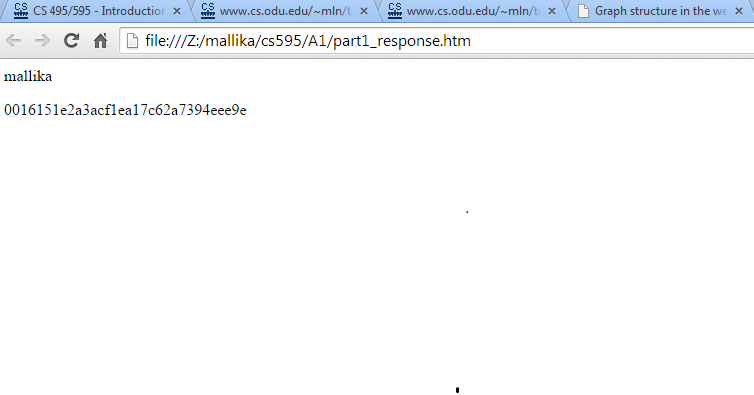
\includegraphics[scale=0.60]{part1_response.png}
        \caption{Response for the curl command}
        \label{fig:X-distribution}
    \end{center}
\end{figure}